\begin{pastexam}[label={px:ncku-106-prog-05}]{成大資訊聯招 106 學年度 第 5 題}
（計算）

(10\%) Given a sequence $K=\langle k_1, k_2,\ldots, k_6\rangle$ of 6 distinct keys in sorted order
with probabilities 0.06, 0.08, 0.10, 0.04, 0.12, 0.14. Some searches may be for values not in $K$,
and so we also have 7 dummy keys, $d_0, d_1,\ldots, d_6$, with probabilities 0.07, 0.07, 0.07, 0.07,
0.06, 0.06, 0.06. Because we have probabilities of searches for each key and each dummy key, we can
determine the expected cost a search in a given binary search tree $T$. Suppose the expected cost
of a search in $T$ is
\[
\text{E[search cost in }T]=\sum_{i=1}^{n}(depth_T(k_i)+1)\cdot p_i+\sum_{i=0}^{n}(depth_T(d_i)+1)\cdot q_i\ ,\ \text{where}
\]
$depth_T$ denotes a node's depth in the tree $T$. Determine the cost of an optimal binary search
tree.
\end{pastexam}

\begin{pastsoln}
答案：最佳二元搜尋樹的期望成本是 $2.99$；樹的根是 $k_3$（畫在最後）。

\textbf{成本模型和資結書的差別。} 題目的成本對虛擬鍵 $d_i$ 也算 $\operatorname{depth}(d_i) + 1$，資結書
第~18.4~節只算 $\operatorname{depth}(d_i)$（走到 $d_i$ 不再比較）。 每棵樹的兩種成本剛好差
$\sum_{i=0}^{6} q_i = 0.46$，是同一個常數，所以最佳的樹一樣，只是數字差 $0.46$。 下面照題目的定義算。
$\sum p_i + \sum q_i = 0.54 + 0.46 = 1$，機率和是 $1$。

\textbf{遞迴式。} 令 $e[i, j]$ 是裝著 $k_i..k_j$（以及 $d_{i-1}..d_j$）的最佳子樹的期望成本，
$w(i, j) = \sum_{l=i}^{j} p_l + \sum_{l=i-1}^{j} q_l$。 把子樹掛到新的根下面，裡面每個節點深度加一，成本
增加 $w$；所以照資結書虛擬碼~18.9 的推導，只有空樹的初值不同（只剩一個虛擬鍵 $d_{i-1}$，成本是
$1 \cdot q_{i-1}$）：
\[
e[i, j] = \begin{cases}
q_{i-1}, & j = i - 1, \\[2pt]
\displaystyle\min_{i \le r \le j} \bigl\{\, e[i, r-1] + e[r+1, j] \,\bigr\} + w(i, j), & i \le j ,
\end{cases}
\]
其中 $w(i, i-1) = q_{i-1}$，$w(i, j) = w(i, j-1) + p_j + q_j$。

\textbf{填表。} 空樹：$e[1,0] = e[2,1] = e[3,2] = e[4,3] = 0.07$，$e[5,4] = e[6,5] = e[7,6] = 0.06$。
一個鍵（$\ell = 1$）時 $w(i, i) = q_{i-1} + p_i + q_i$，$e[i, i] = q_{i-1} + q_i + w(i, i)$：
\begin{center}
\small
\begin{tabular}{ccccccc}
\toprule
$i$ & 1 & 2 & 3 & 4 & 5 & 6 \\
\midrule
$w(i, i)$ & 0.20 & 0.22 & 0.24 & 0.17 & 0.24 & 0.26 \\
$e[i, i]$ & 0.34 & 0.36 & 0.38 & 0.30 & 0.36 & 0.38 \\
\bottomrule
\end{tabular}
\end{center}
$\ell \ge 2$ 的每一格寫出每個 $r$ 的 $e[i, r-1] + e[r+1, j] + w(i, j)$，粗體是最小的：

{\footnotesize
\begin{center}
\begin{tabular}{c c p{0.68\linewidth} c c}
\toprule
$(i, j)$ & $w$ & 每個 $r$ 的成本 & $e$ & $\mathit{root}$ \\
\midrule
$(1,2)$ & 0.35 & $r=1$：$0.07+0.36+0.35=0.78$；$r=2$：$0.34+0.07+0.35=\mathbf{0.76}$ & 0.76 & 2 \\
$(2,3)$ & 0.39 & $r=2$：$0.07+0.38+0.39=0.84$；$r=3$：$0.36+0.07+0.39=\mathbf{0.82}$ & 0.82 & 3 \\
$(3,4)$ & 0.34 & $r=3$：$0.07+0.30+0.34=\mathbf{0.71}$；$r=4$：$0.38+0.06+0.34=0.78$ & 0.71 & 3 \\
$(4,5)$ & 0.35 & $r=4$：$0.07+0.36+0.35=0.78$；$r=5$：$0.30+0.06+0.35=\mathbf{0.71}$ & 0.71 & 5 \\
$(5,6)$ & 0.44 & $r=5$：$0.06+0.38+0.44=0.88$；$r=6$：$0.36+0.06+0.44=\mathbf{0.86}$ & 0.86 & 6 \\
\midrule
$(1,3)$ & 0.52 & $r=1$：$0.07+0.82+0.52=1.41$；$r=2$：$0.34+0.38+0.52=\mathbf{1.24}$；$r=3$：$0.76+0.07+0.52=1.35$ & 1.24 & 2 \\
$(2,4)$ & 0.49 & $r=2$：$0.07+0.71+0.49=1.27$；$r=3$：$0.36+0.30+0.49=\mathbf{1.15}$；$r=4$：$0.82+0.06+0.49=1.37$ & 1.15 & 3 \\
$(3,5)$ & 0.52 & $r=3$：$0.07+0.71+0.52=1.30$；$r=4$：$0.38+0.36+0.52=\mathbf{1.26}$；$r=5$：$0.71+0.06+0.52=1.29$ & 1.26 & 4 \\
$(4,6)$ & 0.55 & $r=4$：$0.07+0.86+0.55=1.48$；$r=5$：$0.30+0.38+0.55=\mathbf{1.23}$；$r=6$：$0.71+0.06+0.55=1.32$ & 1.23 & 5 \\
\midrule
$(1,4)$ & 0.62 & $r=1$：$0.07+1.15+0.62=1.84$；$r=2$：$0.34+0.71+0.62=\mathbf{1.67}$；$r=3$：$0.76+0.30+0.62=1.68$；$r=4$：$1.24+0.06+0.62=1.92$ & 1.67 & 2 \\
$(2,5)$ & 0.67 & $r=2$：$0.07+1.26+0.67=2.00$；$r=3$：$0.36+0.71+0.67=\mathbf{1.74}$；$r=4$：$0.82+0.36+0.67=1.85$；$r=5$：$1.15+0.06+0.67=1.88$ & 1.74 & 3 \\
$(3,6)$ & 0.72 & $r=3$：$0.07+1.23+0.72=2.02$；$r=4$：$0.38+0.86+0.72=1.96$；$r=5$：$0.71+0.38+0.72=\mathbf{1.81}$；$r=6$：$1.26+0.06+0.72=2.04$ & 1.81 & 5 \\
\midrule
$(1,5)$ & 0.80 & $r=1$：$0.07+1.74+0.80=2.61$；$r=2$：$0.34+1.26+0.80=2.40$；$r=3$：$0.76+0.71+0.80=\mathbf{2.27}$；$r=4$：$1.24+0.36+0.80=2.40$；$r=5$：$1.67+0.06+0.80=2.53$ & 2.27 & 3 \\
$(2,6)$ & 0.87 & $r=2$：$0.07+1.81+0.87=2.75$；$r=3$：$0.36+1.23+0.87=2.46$；$r=4$：$0.82+0.86+0.87=2.55$；$r=5$：$1.15+0.38+0.87=\mathbf{2.40}$；$r=6$：$1.74+0.06+0.87=2.67$ & 2.40 & 5 \\
\midrule
$(1,6)$ & 1.00 & $r=1$：$0.07+2.40+1.00=3.47$；$r=2$：$0.34+1.81+1.00=3.15$；$r=3$：$0.76+1.23+1.00=\mathbf{2.99}$；$r=4$：$1.24+0.86+1.00=3.10$；$r=5$：$1.67+0.38+1.00=3.05$；$r=6$：$2.27+0.06+1.00=3.33$ & 2.99 & 3 \\
\bottomrule
\end{tabular}
\end{center}
}

每一格的最小值都只有一個 $r$ 取到，最佳樹唯一。 $e[1, 6] = 2.99$ 就是答案。

\textbf{還原樹。} $\mathit{root}[1,6] = 3$：根是 $k_3$，左邊 $k_1..k_2$、右邊 $k_4..k_6$。 $\mathit{root}[1,2] = 2$：
$k_2$ 的左子是 $k_1$（$\mathit{root}[1,1] = 1$），右邊是虛擬鍵 $d_2$。 $\mathit{root}[4,6] = 5$：$k_5$ 的左子是
$k_4$、右子是 $k_6$。

\begin{center}
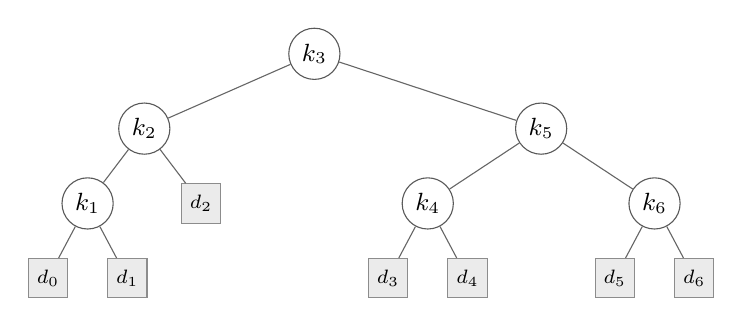
\begin{tikzpicture}[x=0.72cm, y=0.95cm,
    key/.style={circle, draw=black!65, minimum size=6.5mm, inner sep=0pt, font=\small},
    ext/.style={rectangle, draw=black!45, fill=black!8, minimum size=5mm, inner sep=1pt, font=\scriptsize},
    ed/.style={draw=black!60}]
\node[key] (k3) at (5,0) {$k_3$};
\node[key] (k2) at (2,-1) {$k_2$};
\node[key] (k5) at (9,-1) {$k_5$};
\node[key] (k1) at (1,-2) {$k_1$};
\node[ext] (d2) at (3,-2) {$d_2$};
\node[key] (k4) at (7,-2) {$k_4$};
\node[key] (k6) at (11,-2) {$k_6$};
\node[ext] (d0) at (0.3,-3) {$d_0$};
\node[ext] (d1) at (1.7,-3) {$d_1$};
\node[ext] (d3) at (6.3,-3) {$d_3$};
\node[ext] (d4) at (7.7,-3) {$d_4$};
\node[ext] (d5) at (10.3,-3) {$d_5$};
\node[ext] (d6) at (11.7,-3) {$d_6$};
\draw[ed] (k3) -- (k2); \draw[ed] (k3) -- (k5);
\draw[ed] (k2) -- (k1); \draw[ed] (k2) -- (d2);
\draw[ed] (k5) -- (k4); \draw[ed] (k5) -- (k6);
\draw[ed] (k1) -- (d0); \draw[ed] (k1) -- (d1);
\draw[ed] (k4) -- (d3); \draw[ed] (k4) -- (d4);
\draw[ed] (k6) -- (d5); \draw[ed] (k6) -- (d6);
\end{tikzpicture}
\end{center}

\textbf{直接算這棵樹的成本核對。} 每個節點的（深度 $+ 1$）乘上機率：
\begin{center}
\small
\begin{tabular}{l*{13}{c}}
\toprule
節點 & $d_0$ & $k_1$ & $d_1$ & $k_2$ & $d_2$ & $k_3$ & $d_3$ & $k_4$ & $d_4$ & $k_5$ & $d_5$ & $k_6$ & $d_6$ \\
\midrule
深度 $+1$ & 4 & 3 & 4 & 2 & 3 & 1 & 4 & 3 & 4 & 2 & 4 & 3 & 4 \\
機率 & .07 & .06 & .07 & .08 & .07 & .10 & .07 & .04 & .06 & .12 & .06 & .14 & .06 \\
乘積 & .28 & .18 & .28 & .16 & .21 & .10 & .28 & .12 & .24 & .24 & .24 & .42 & .24 \\
\bottomrule
\end{tabular}
\end{center}
加起來 $0.28 + 0.18 + 0.28 + 0.16 + 0.21 + 0.10 + 0.28 + 0.12 + 0.24 + 0.24 + 0.24 + 0.42 + 0.24 = 2.99$，
和表格的 $e[1, 6]$ 相同。 照資結書的成本模型（虛擬鍵不加一），同一棵樹的成本是 $2.99 - 0.46 = 2.53$。
\end{pastsoln}
